\documentclass[12pt,a4paper,titlepage,oneside]{article}
\usepackage{report}
\usepackage{graphicx}
\usepackage{url}
\usepackage{amsmath}
\usepackage{amssymb}
\usepackage{textcomp}
\usepackage{color}

\definecolor{mygreen}{rgb}{0.133,0.545,0.133}
\definecolor{mygray}{rgb}{0.5,0.5,0.5}
\definecolor{mymauve}{rgb}{0.627,0.126,0.941}

\title{Assignment 1}

\author{Konstantin Selyunin, \matrnr 1228206   \\
         {\small e1228206@student.tuwien.ac.at} \\
        Vorname2 Nachname2, \matrnr 99012345 \\
         {\small e99012345@student.tuwien.ac.at}
}
\begin{document}

% create titlepage
\maketitle

%\tableofcontents
%\newpage

%------------------------------------------------------------------
\section{Problem 1}

\subsection{Problem Statement}
\label{problem:1}

In directory \texttt{insertion\_sort}, implement the function
\texttt{main.c:run()}. This routine should call the insertion
sort routine several times, with different arrays of size $32$.

\begin{itemize}
\item[Q1:] What is the minimum and maximum number of times the statement
           labeled \texttt{insertion\_sort\_move} might be
           executed for some input data (assuming an array size of $N$)?
\item[Q2:] How many test runs do you need to cover all possible paths through
           the function?
\item[Q3:] Report the minimum and maximum execution times measured for
           your test runs of insertion sort.
\end{itemize}


\subsection{Solution}
% TODO
\begin{itemize}
\item[A1:]
For an array of size $N$ the labeled statement
\texttt{insertion\_sort\_move} might be executed from $0$ (sorted) to
$N\times(N-1)/2$ (reverse order) times (in our case for an array of 32 
elements from 0 to 496). 

\item[A2:] 

  Assume that the length of the input array is $N$.

  After an inspection of the sorting algorithm one can see that the
  algoritm behaviour does not depend on the exact values of the input
  array.
  It only depends on the relations between the array elements.
  The reason is that the array elements are only compared by
  relational operarors like ``$>$'' and the only operation invoked on
  array elements is copying.
  This means that control-flow path is the same for two arrays of
  lenght $N$ with the same distribution of elements inversions.

  In the very general case two arbitrary elements $a$ and $b$ of the
  input array can be related as $a<b$, $a=b$ or $a>b$, and the
  execution path might be influenced by this fact in three different
  ways.
  The total number of permutations, that take into account equalities
  and inversions, for arrays of length $N$ can be expressed as

  \begin{equation}
	\sum_{n=1}^N \ \ \sum_{\substack{
	  \bigwedge_{i=1}^n m_i \geq 1 
	  \\ \sum_{i=1}^n m_i = N}} \binom N {m_1, m_2, \ldots, m_n}.
	  \label{equ:genpath}
	\end{equation}

	Potentially, each of these arrays might cause a sorting algorithm
	to follow a unique execution path.
	However, in the case of insertion sort algorithm we know that
	relations $a<b$ and $a=b$ cannot be distinguished.
	This reduces the number of paths accordint to~(\ref{equ:genpath})
	to the number of $N!$.
	A simpler explanation can be provided in this case.
	When the insertion sort algorithm processes the element at the
	position~$i$ ($1 \leq i \leq N$), all the elements at the previous
	positions $1\ldots i-1$ are already sorted.
	For the element $i$ there are now exactly $i$ positions to be
	placed.
	This adds a factor $i$ to the number of total pths that should be
	executed.
	Hence, we get for the total number of path an expression

	%\begin{equation}
	$$
	  \prod_{i=1}^N i = N!.
	$$
	%\end{equation}

           
\item[A3:] 
The minimum execution time (in processor cycles) is $t_1 = 5477$
for the sorted array, the maximum is $t_2 = 30083$ for elements in
reverse order as well as for an array of equal elements (e.g. all
zeros). Sorting an array of random elements takes `usually' 17/18k cycles.
For details see Figure~\ref{fig:opt_compare}.

\end{itemize}

\subsection{Listings}
% TODO
\subsubsection{\texttt{main.c:run()}}
\lstset{ %
  language=C,                 	   % the language of the code
  backgroundcolor=\color{white},   % choose the background color; you must add \usepackage{color} or \usepackage{xcolor}
  basicstyle=\footnotesize\ttfamily,        % the size of the fonts that are used for the code
  breakatwhitespace=false,         % sets if automatic breaks should only happen at whitespace
  breaklines=true,                 % sets automatic line breaking
  captionpos=b,                    % sets the caption-position to bottom
  commentstyle=\color{mygreen},    % comment style
  deletekeywords={...},            % if you want to delete keywords from the given language
  escapeinside={\%*}{*)},          % if you want to add LaTeX within your code
  extendedchars=true,              % lets you use non-ASCII characters; for 8-bits encodings only, does not work with UTF-8
  %frame=single,                    % adds a frame around the code
  keepspaces=true,                 % keeps spaces in text, useful for keeping indentation of code (possibly needs columns=flexible)
  keywordstyle=\bfseries\color{blue},       % keyword style
  morekeywords={*,...},            % if you want to add more keywords to the set
  numbers=left,                    % where to put the line-numbers; possible values are (none, left, right)
  numbersep=5pt,                   % how far the line-numbers are from the code
  numberstyle=\tiny\color{mygray}, % the style that is used for the line-numbers
  rulecolor=\color{black},         % if not set, the frame-color may be changed on line-breaks within not-black text (e.g. comments (green here))
  showspaces=false,                % show spaces everywhere adding particular underscores; it overrides 'showstringspaces'
  showstringspaces=false,          % underline spaces within strings only
  showtabs=false,                  % show tabs within strings adding particular underscores
  stepnumber=1,                    % the step between two line-numbers. If it's 1, each line will be numbered
  stringstyle=\color{mymauve},     % string literal style
  tabsize=2,                       % sets default tabsize to 2 spaces
  %extendedchars=true,
  %aboveskip={1.5\baselineskip},
  %columns=fixed, upquote=true,
  %title=\lstname                   % show the filename of files included with \lstinputlisting; also try caption instead of title
}


\lstinputlisting{src/main.c}

%------------------------------------------------------------------
\newpage
\section{Problem 2}

\subsection{Problem Statement}
\label{problem:2}

Add loop bounds and additional flow facts for
\texttt{insertion\_sort.c:insertion\_sort()}, and analyze the WCET of
\texttt{insertion\_sort}.

\begin{itemize}

\item[Q1:]
  What is the WCET of insertion\_sort, assuming the array has 8,16,32 or 64
  elements? Compare the WCET for arrays of size $32$ with your measurement
  results.

\item[Q2:]
  What other properties of the input (despite the size of the array) have a
  significant impact on the execution time? How could you take them into
  account during static WCET analysis?

\item[Q3:]
  Now try compiling with \texttt{-O1} (cf.\ the Makefile).  Try to add your
  flow facts for array size $32$.  This might require a different method than
  source code annotations.  List the maximally observed execution time and the
  WCET from analysis, and compare them to the results obtained with
  \texttt{-O0}.

\item[Q4:] (Bonus)
  Figure~\ref{fig:cfg.insertion_sort} depicts the \emph{control-flow graph}
  (CFG) of the \texttt{insertion\_sort} function as exported from the compiler
  intermediate representation.
  %
  Formulate an ILP problem to calculate the WCET.  That is, specify a set of
  (integer) variables, a linear objective function, and a set of linear
  constraints, such that the solution to the problem is an upper bound for the
  execution time of the program.  The linear constraints consist of the
  structural constraints given by the CFG and the flow constraints you
  specified.
  For the basic block costs, assume a very simple model and use the costs
  given in Table~\ref{tab:cfg.insertion_sort}.
  Write an input file for an ILP solver%
  \footnote{Recommendation: \url{http://sourceforge.net/projects/lpsolve}},
  and check the solution calculated by the solver.
  Do not forget to give the number of times each basic block is executed in
  your solution.

\end{itemize}


\begin{figure}
  \centering
  \begin{minipage}[c]{.6\linewidth}
    %\vspace{0pt}
    \centering
    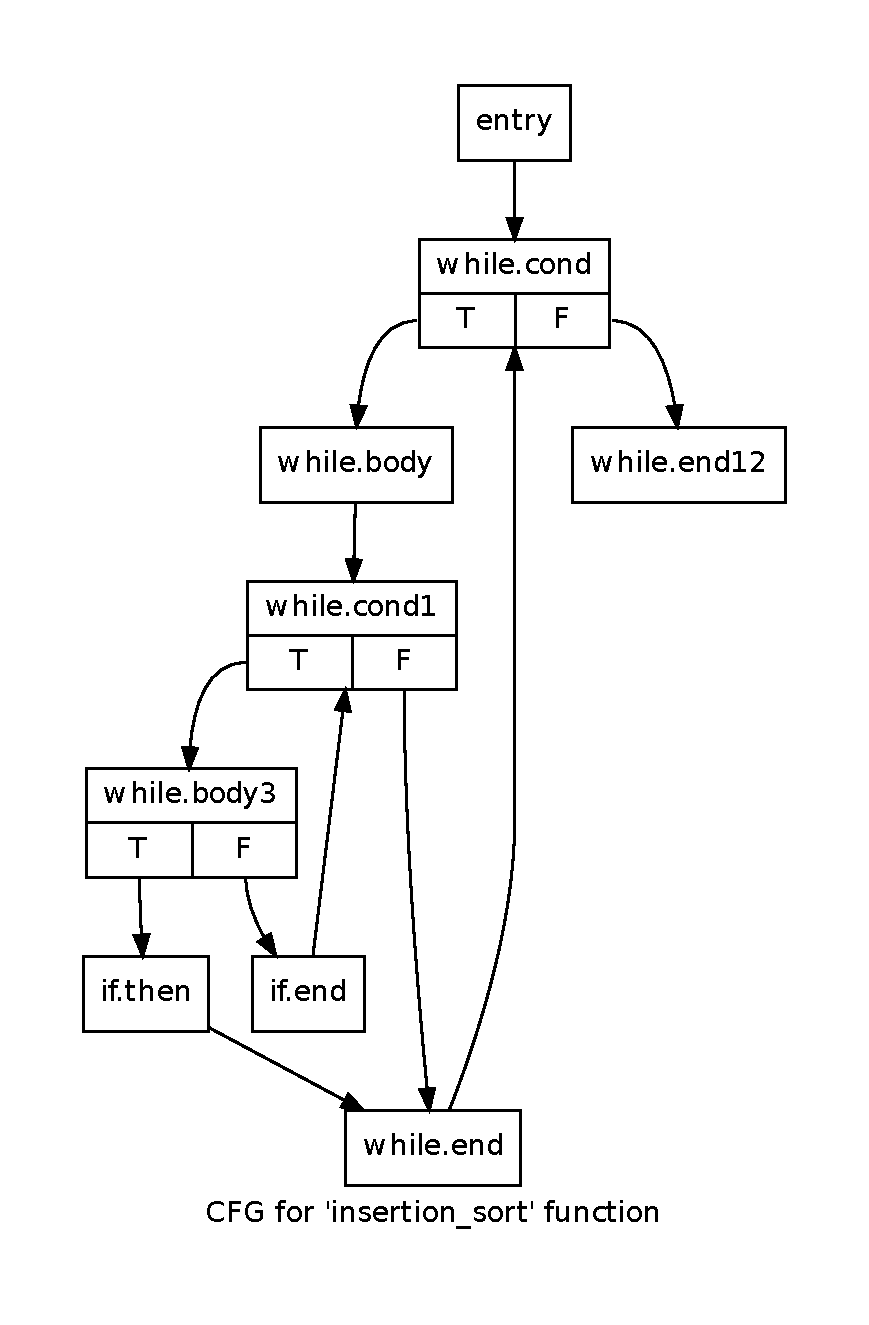
\includegraphics[width=0.90\linewidth]{../assignment/cfg_insertion_sort}
  \end{minipage}%
  \begin{minipage}[c]{.3\linewidth}
    %\vspace{0pt}
    \centering
    \small
    \begin{tabular}{|l|r|}
      \hline
      Basic Block & Cost \\
      \hline
      entry & 12 \\
      while.cond & 6 \\
      while.body & 15 \\
      while.cond1 & 4 \\
      while.body3 & 11 \\
      if.then & 1 \\
      if.end & 21 \\
      while.end & 16 \\
      while.end12 & 1 \\
      \hline
    \end{tabular}
  \end{minipage}
  \caption{Control-Flow Graph for \texttt{insertion\_sort} (from LLVM IR)
           and costs for the execution of basic blocks.}
  \label{fig:cfg.insertion_sort}
\end{figure}

\clearpage


\subsection{Solution}
% TODO

\begin{itemize}

\item[A1:]

The results of WCET static analysis, obtained with \texttt{a3patmos}
tool (column 2), are summarized in the table below:

\begin{tabular}{ | r | r | r |}
\hline
Array size & WCET (cycles) & Measured \\\hline
8  & 6512 & - \\\hline
16 & 22888 & - \\\hline
32 & 46904 & 30083 \\\hline
64 & 330808 & - \\\hline
\end{tabular}

For an array of 32 elements \texttt{a3patmos} gives result which is
approximately 1.5 times larger then the largest measurement. 
If the 'triangulation' structure of the loops is not
imposed as a constraint, the result is even more
pessimistic (85.5k cycles for array size of 32).

\item[A2:]
Number of inversions in the input array has significant impact on
the execution time. In order to take it into
account during static WCET analysis, we add linear
constraint for maximum number of inversions in the inner loop.

\item[A3:]
For this task we modify \texttt{Makefile} and include corresponding
\texttt{insertion\_sort\_O1.*} targets.
We also define annotations in a separate file (aiT.ais, see listing or supplement).
The differences between execution times for the test cases 
and the WCET are summarized in the Figure~\ref{fig:opt_compare}.
Optimizations performed by compiler  reduce execution
time by approximately factor of 3. The pitfall here is
that the control flow graph from \texttt{a3patmos} tool does not give 
the valid addresses of instructions corresponding to \texttt{insertion\_sort\_move}:
to solve this issue we obtain the addresses from the disassembly file
(after analysing \texttt{insertion\_sort} assembly code).


\begin{figure}%[hb!]
  \centering
  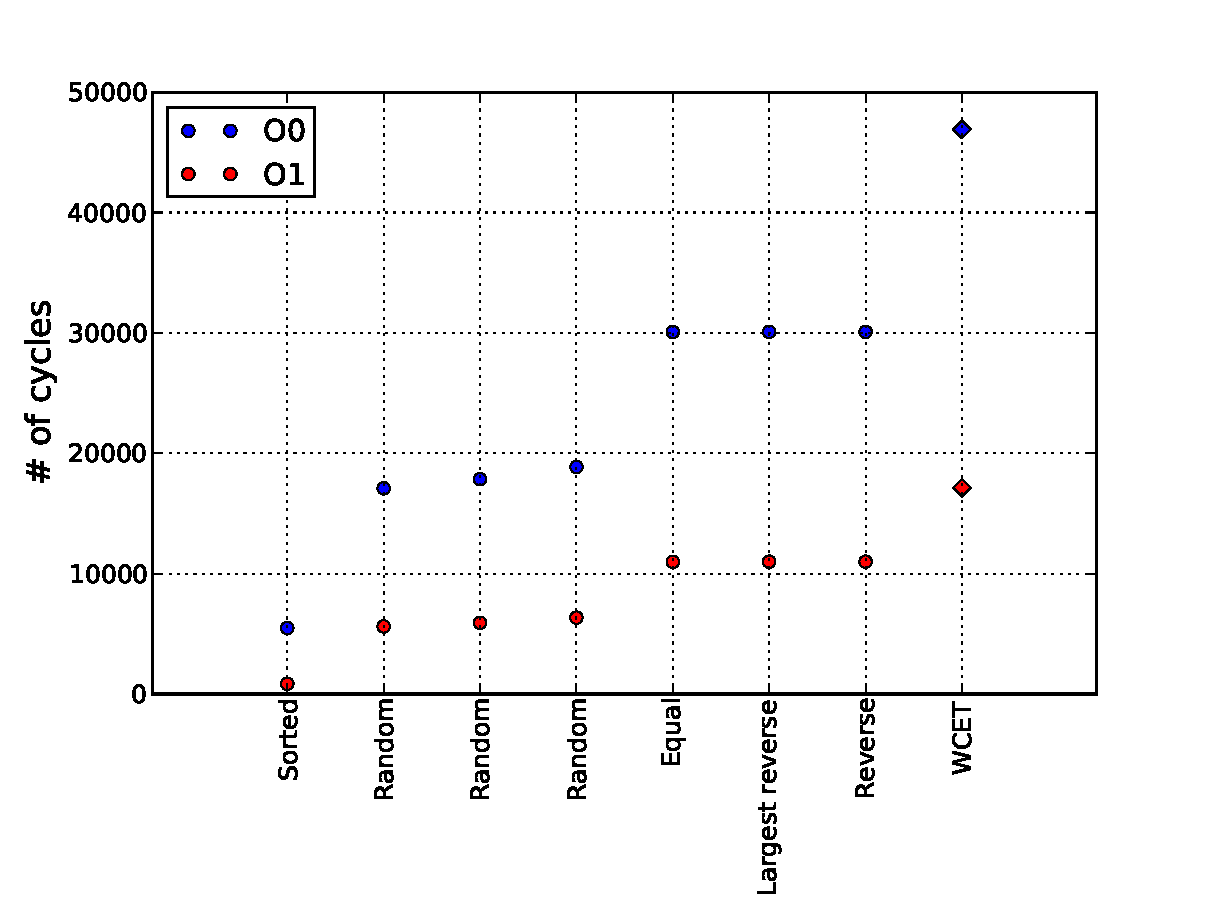
\includegraphics[width=4in]{q2_3}
  \caption
  {Execution time measurements and the WCET for \texttt{-O0} and
  \texttt{-O1}}
	\label{fig:opt_compare}
\end{figure}


\item[A4:] 
In order to perform the analysis we build a directed graph that assigns execution time to edges but not vertices~(Fig.~\ref{fig:ilp}).
This is done by moving execution time from each block (corresponding to a vertex) to its outgoing edges.
The same value (equal to the corresponding block execution cost) is assigned to all outgoing edges.
Since we do not have outgoing edges form the block \texttt{while.end12}, we add one more vertex to the graph (which we call \texttt{exit}) and an edge between vertices \texttt{while.end12} and \texttt{exit}.
The cost of \texttt{while.end12} block is assigned to the new edge.
\begin{figure}
  \centering
  \begin{minipage}[c]{.6\linewidth}
    \centering
    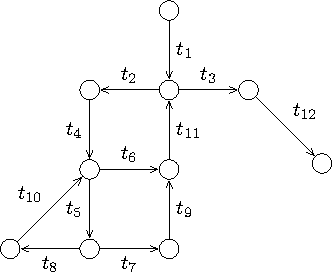
\includegraphics[width=0.8\textwidth]{graph}
  \end{minipage}%
  \begin{minipage}[c]{.3\linewidth}
    \centering
    \small
	\begin{tabular}{l|l}
		\hline
		Edge Cost & Basic Block \\
		\hline
		$t_1$ & entry \\
		$t_2 = t_3$ & while.cond \\
		$t_4$ & while.body \\
		$t_5 = t_6$ & while.cond1 \\
		$t_7 = t_8$ & while.body3 \\
		$t_9$ & if.then \\
		$t_{10}$ & if.end \\
		$t_{11}$ & while.end \\
		$t_{12}$ & while.end12 \\
		\hline
	\end{tabular}
  \end{minipage}
  \caption{Control-Flow Graph for ILP problem formulation}
  \label{fig:ilp}
\end{figure}

A cost value and a number of executions is associated with each edge of the graph, such that the edge $i$ has the cost $t_i$ and the number of executions $x_i$ correspondingly.
The ILP problem consists of the objective function and the constraints.
The objective function is maximization of the execution time:
\begin{equation}
\max_{x_1, x_2, \ldots x_{12}} \ \sum_{i=1}^{12} x_i t_i.
\label{equ:objective}
\end{equation}

The constraints reflect the facts we know about control-flow of the function.
The node constraints describe the fact that each program block is entered and left exactly the same number of times:
\begin{equation}
	\left.\begin{aligned}
		x_2 + x_3	&= x_1 + x_{11}\\
		x_2			&= x_4\\
		x_4 + x_{10}	&= x_5 + x_6\\
		x_5			&= x_7 + x_8\\
		x_7			&= x_9\\
		x_8			&= x_{10}\\
		x_6 + x_9	&= x_{11}\\
		x_3			&= x_{12}
	\end{aligned}\right.
\label{equ:node}
\end{equation}
This control flow constraints itself cannot give a finite solution because of cycles in the graph.
Thus, we add a requirement of a single function entrance and function exit or infinite looping:
\begin{equation}
	\left.\begin{aligned}
		x_1			&= 1\\
		x_{12}		&\leq 1
	\end{aligned}\right.
\label{equ:single}
\end{equation}
This additional requirements still do not make the solution finite.
We should add the constraints that describe loop bounds.
We suppose that the length of the input array is $N$.
From the previously done analysis we know that in this case the outer loop is executed exactly $N$ times and the inner loop---not more than $N(N-1)/2$.
Hence, we add
\begin{equation}
	\left.\begin{aligned}
		x_{11}		&= N\\
		x_{10}		&\leq N(N-1)/2
	\end{aligned}\right.
\label{equ:loops}
\end{equation}
Finally, there are physical feasibility constraints:
\begin{equation}
		x_i \in \mathbb{N}, \quad \mathrm{where}\ 1 \leq i \leq 12
\label{equ:feasibility}
\end{equation}
All the constraints (\ref{equ:objective}--\ref{equ:feasibility}) formulate the ILP problem for IPET analysis.
Equation (\ref{equ:feasibility}) should be passed to the solver through the type information, i.e. the solver will treat the variables as natural numbers implicitly.

The problem can be solved every time for each specific $N$ and $t_{1} \ldots t_{12}$.
However, the intuition and previous analysis say that the WCET should always correspond to the case when the inner loop is executed $N(N-1)/2$ times.
Since the problem is not large, we can try to prove it analytically.

First of all, eliminate the redundant variables in node constraints:
\begin{equation}
	\left.\begin{aligned}
		x_2 + x_3	&= 1 + N\\
		x_2 + x_8	&= x_5 + x_6\\
		x_5			&= x_7 + x_8\\
		x_6 + x_7	&= N\\
	\end{aligned}\right.
\label{equ:node_simpl}
\end{equation}
and prove termination of the \texttt{insertion\_sort} function.
Termination is formulated as $x_{12} = 1$.
From $x_3 = x_{12}$ and $x_{12} \leq 1$ we conclude $x_3 \leq 1$, i.e. we should prove that $x_3 = 1$ but not $x_3 = 0$.

Suppose that $x_3 = 0$.
From (\ref{equ:node_simpl}) we have
\begin{equation*}
	\left\{\begin{aligned}
		x_2			&= 1 + N\\
		x_2 + x_8	&= x_5 + x_6\\
		x_5			&= x_7 + x_8\\
		x_6 + x_7	&= N\\
	\end{aligned}\right.
\Rightarrow
	\left\{\begin{aligned}
		1 + N + x_8	&= x_7 + x_8 + x_6\\
		x_6 + x_7	&= N\\
	\end{aligned}\right.
\Rightarrow
	\left\{\begin{aligned}
		x_6 + x_7 	&= N+1\\
		x_6 + x_7	&= N\\
	\end{aligned}\right.
\end{equation*}
which is a contradiction.
Thus, $x_3 = x_{12} = 1$.
Taking this into account and $x_8 = x_{10} \leq N(N-1)/2$ we can further reduce our set of constraints.
Additionally, we can remove constants from the objective function.
After simplification the ILP problem looks as
\begin{equation}
\begin{aligned}
	\max_{x_5, x_6, x_7, x_8} \left(t_5 x_5 + t_5 x_6 + (t_7+t_9)x_7 + (t_7+t_{10}) x_8 \right)\\
	\left.\begin{aligned}
		N + x_8		&= x_5 + x_6\\
		x_5			&= x_7 + x_8\\
		x_6 + x_7	&= N\\
		x_8			&\leq N(N-1)/2
	\end{aligned}\right.
\end{aligned}
\label{equ:ilp}
\end{equation}
and we know that $x_1 = x_3 = x_{12} = 1$, $x_2 = x_4 = x_{11} = N$, $x_9 = x_7$ and $x_{10} = x_8$.

Suppose that we have a solution $\{x_5, x_6, x_7, x_8\}$ of (\ref{equ:ilp}), for which $x_8 < N(N-1)/2$.
One can easily see that this solution is not the optimal.
The solution $\{x'_5 = x_5+1, x'_6 = x_6, x'_7 = x_7, x'_8 = x_8+1\}$ gives a larger value of the optimization function under assumption $t_5 + t_7 + t_{10} > 0$.
For any realistic implementation the assumption is true.
We can increment $x_5$ and $x_8$ until $x_8 = N(N-1)/2$.
And this will give the maximum value of the optimization function for any particular $x_6$ and $x_7$.
Thus, we conclude $x_8 = N(N-1)/2$.

Now the ILP problem looks as 
\begin{equation}
\begin{aligned}
	\max_{x_5, x_6, x_7} \left(t_5 x_5 + t_5 x_6 + (t_7+t_9)x_7 \right)\\
	\left.\begin{aligned}
		N + N(N-1)/2	&= x_5 + x_6\\
		x_5			&= x_7 + N(N-1)/2\\
		x_6 + x_7	&= N\\
	\end{aligned}\right.
\end{aligned}
\label{equ:ilp2}
\end{equation}
where the last constraint is redundant (it is a sum of two other constraints).

To solve problem (\ref{equ:ilp2}) we express
\begin{equation*}
	\left.\begin{aligned}
		x_6 = N(N+1)/2 - x_5\\
		x_7 = x_5 - N(N-1)/2
	\end{aligned}\right.
\end{equation*}
and put it to the optimization function:
\begin{equation*}
	\left.\begin{aligned}
		\max_{x_5, x_6, x_7, x_8} \left(t_5x_5 + t_5x_6 + (t_7+t_9)x_7\right) =\\
		\max_{x_5} \left(t_5x_5 + t_5\left(\frac{N(N+1)}2 - x_5\right) + (t_7+t_9)\left(x_5 - \frac{N(N-1)}2\right)\right) \sim\\
		\max_{x_5} \left(t_5x_5 - t_5x_5 + (t_7+t_9)x_5\right) =\\
		\max_{x_5} \left((t_7+t_9)x_5\right) \sim\\
		\max_{x_5} x_5
	\end{aligned}\right.
\end{equation*}
under assumption $t_7+t_9 > 0$, which is true for any realistic implementation.

In order to maximize our optimization function we should maximize $x_5$, but this is infinity.
At this point the feasibility constraint $x_6 \geq 0$ comes into a play:
\begin{equation*}
x_6 = N(N+1)/2 - x_5 \geq 0
\quad\Rightarrow\quad
x_5 \leq N(N+1)/2
\end{equation*}
Clearly, the maximal possible value of $x_5$ is $N(N+1)/2$.
Finally, we find $x_6 = 0$, $x_7 = N$.

Our solution looks as following\\
\begin{tabular}{c|c|c|c|c|c|c|c|c|c|c|c}
\hline
$x_1$ & $x_2$ & $x_3$ & $x_4$ & $x_5$ & $x_6$ & $x_7$ & $x_8$ & $x_9$ & $x_{10}$ & $x_{11}$ & $x_{12}$ \\
\hline
%$1$ & $N$ & $1$ & $N$ & $N(N+1)/2$ & $0$ & $N$ & $N(N-1)/2$ & $N$ & $N(N-1)/2$ & $N$ & $1$ \\
$1$ & $N$ & $1$ & $N$ & $\frac{N(N+1)}2$ & $0$ & $N$ & $\frac{N(N-1)}2$ & $N$ & $\frac{N(N-1)}2$ & $N$ & $1$ \\
\hline
\end{tabular}\\
and the WCET is $\sum_{i=1}^{12} x_i t_i$.
The solution does not depend on the exact values of $t_1, t_2, \ldots t_{12}$, only assumptions $t_5 + t_7 + t_{10} > 0$ and $t_7+t_9 > 0$ are important.
For $N=32$ and cost values given in Fig.~\ref{fig:cfg.insertion_sort} the solution is\\
\begin{tabular}{c|c|c|c|c|c|c|c|c|c|c|c|c}
\hline
$x_1$ & $x_2$ & $x_3$ & $x_4$ & $x_5$ & $x_6$ & $x_7$ & $x_8$ & $x_9$ & $x_{10}$ & $x_{11}$ & $x_{12}$ & WCET\\
\hline
1 & 32 & 1 & 32 & 528 & 0 & 32 & 496 & 32 & 496 & 32 & 1  & 19571\\
\hline
\end{tabular}\\
The same values were obtaines with the \texttt{lp\_solve} solver that was run on the originaly composed constraints (\ref{equ:objective}--\ref{equ:feasibility}).

\end{itemize}



\subsection{Listings}

\subsubsection{\texttt{*.ais} files for arrays of different size}
\textbf{Array size 8}
\lstset{ %
  language=python,                 	   % the language of the code
  backgroundcolor=\color{white},   % choose the background color; you must add \usepackage{color} or \usepackage{xcolor}
  basicstyle=\footnotesize\ttfamily,        % the size of the fonts that are used for the code
  breakatwhitespace=false,         % sets if automatic breaks should only happen at whitespace
  breaklines=true,                 % sets automatic line breaking
  captionpos=b,                    % sets the caption-position to bottom
  commentstyle=\color{mygray},    % comment style
  deletekeywords={...,in},            % if you want to delete keywords from the given language
  escapeinside={\%*}{*)},          % if you want to add LaTeX within your code
  extendedchars=true,              % lets you use non-ASCII characters; for 8-bits encodings only, does not work with UTF-8
  %frame=single,                    % adds a frame around the code
  keepspaces=true,                 % keeps spaces in text, useful for keeping indentation of code (possibly needs columns=flexible)
  keywordstyle=\bfseries\color{blue},       % keyword style
  morekeywords={*,...,instruction,loop, entered, with, max, flow, label},            % if you want to add more keywords to the set
  numbers=left,                    % where to put the line-numbers; possible values are (none, left, right)
  numbersep=5pt,                   % how far the line-numbers are from the code
  numberstyle=\tiny\color{mygray}, % the style that is used for the line-numbers
  rulecolor=\color{black},         % if not set, the frame-color may be changed on line-breaks within not-black text (e.g. comments (green here))
  showspaces=false,                % show spaces everywhere adding particular underscores; it overrides 'showstringspaces'
  showstringspaces=false,          % underline spaces within strings only
  showtabs=false,                  % show tabs within strings adding particular underscores
  stepnumber=1,                    % the step between two line-numbers. If it's 1, each line will be numbered
  stringstyle=\color{mymauve},     % string literal style
  tabsize=2,                       % sets default tabsize to 2 spaces
  %extendedchars=true,
  %aboveskip={1.5\baselineskip},
  %columns=fixed, upquote=true,
  %title=\lstname                   % show the filename of files included with \lstinputlisting; also try caption instead of title
}


\lstinputlisting{src/aiTinsertionSort8.ais}
\textbf{Array size 16}
\lstinputlisting{src/aiTinsertionSort16.ais}
\textbf{Array size 32}
\lstinputlisting{src/aiTinsertionSort32.ais}
\textbf{Array size 64}
\lstinputlisting{src/aiTinsertionSort64.ais}

\subsubsection{}
No listing for this question

\subsubsection{\texttt{-O1}}
\lstinputlisting{src/aiTinsertionSortO1.ais}

\subsubsection{Input file for ILP solver}
\lstset{ %
  language=C,                 	   % the language of the code
  backgroundcolor=\color{white},   % choose the background color; you must add \usepackage{color} or \usepackage{xcolor}
  basicstyle=\footnotesize\ttfamily,        % the size of the fonts that are used for the code
  breakatwhitespace=false,         % sets if automatic breaks should only happen at whitespace
  breaklines=true,                 % sets automatic line breaking
  captionpos=b,                    % sets the caption-position to bottom
  commentstyle=\color{mygreen},    % comment style
  deletekeywords={...},            % if you want to delete keywords from the given language
  escapeinside={\%*}{*)},          % if you want to add LaTeX within your code
  extendedchars=true,              % lets you use non-ASCII characters; for 8-bits encodings only, does not work with UTF-8
  %frame=single,                    % adds a frame around the code
  keepspaces=true,                 % keeps spaces in text, useful for keeping indentation of code (possibly needs columns=flexible)
  keywordstyle=\bfseries\color{blue},       % keyword style
  morekeywords={*,..., max},            % if you want to add more keywords to the set
  numbers=left,                    % where to put the line-numbers; possible values are (none, left, right)
  numbersep=5pt,                   % how far the line-numbers are from the code
  numberstyle=\tiny\color{mygray}, % the style that is used for the line-numbers
  rulecolor=\color{black},         % if not set, the frame-color may be changed on line-breaks within not-black text (e.g. comments (green here))
  showspaces=false,                % show spaces everywhere adding particular underscores; it overrides 'showstringspaces'
  showstringspaces=false,          % underline spaces within strings only
  showtabs=false,                  % show tabs within strings adding particular underscores
  stepnumber=1,                    % the step between two line-numbers. If it's 1, each line will be numbered
  stringstyle=\color{mymauve},     % string literal style
  tabsize=2,                       % sets default tabsize to 2 spaces
  %extendedchars=true,
  %aboveskip={1.5\baselineskip},
  %columns=fixed, upquote=true,
  %title=\lstname                   % show the filename of files included with \lstinputlisting; also try caption instead of title
}

\lstinputlisting{src/p2q4.lp}


%------------------------------------------------------------------
\newpage
\section{Problem 3}

\subsection{Problem Statement}
\label{problem:3}

First, focus on the analysis of \texttt{task.c:merge\_samples()}.  The loop
bounds in this function depend on the input-data dependent parameter
\texttt{@inputcount}, defined to be the maximal value of
\texttt{input->input\_count}. Add loop bounds and flow facts for
\texttt{merge\_samples}, and analyze its WCET assuming that
$\texttt{@inputcount} \leq 64$.

\begin{itemize}

\item[Q1:]
  Describe and justify the loop bounds and flow facts used in the WCET analysis
  of \texttt{merge\_samples}.

\item[Q2:]
  What is the maximum execution time observed for this function? What is the
  analyzed WCET? In case they do not coincide, discuss reasons for the
  impreciseness in the static analysis.

\item[Hint:]
  For measurements, you might want to rely on or start with the test bench
  implemented in\\
  \texttt{main.c:test\_merge\_samples()}.

\item[Hint:]
  Division is implemented in software for the Patmos architecture. We replaced
  the division in the interpolation routine by a lookup table for small values,
  to simplify the analysis problem. You do not need to worry about the analysis
  of \texttt{iinterpolate16}; simply use the following annotations:

\end{itemize}

\begin{verbatim}
  include "llvm.ais";
  instruction "iinterpolate16" + 1 calls is never executed;
  instruction "iinterpolate16" + 2 calls is never executed;
\end{verbatim}


\subsection{Solution}
\begin{itemize}

\item[A1:]
  To justify flow and loop constraints for
  \texttt{merge\_samples} we first need to state the following facts:
  number of samples that are used for analysis is 64
  (\texttt{SAMPLE\_COUNT}). At most 4 consecutive samples could be
  missing (\texttt{MAX\_CONSECUTIVE\_MISSING}). This means that
  minimum number of valid samples to perform the analysis is:
  $${\text{MIN}_\text{valid samples}}  = \lceil\frac{\texttt{SAMPLE\_COUNT}}{\texttt{MAX\_CONSECUTIVE\_MISSING} + 1}\rceil$$
  (in our case 13).
  
  \texttt{merge\_samples} has two nested loops and two conditional
  branches of interest (we do not consider the case when number of
  samples <= 0, where we exit without performing interpolation).

  The outer loop is executed for each sample (either valid or missing,
  64 times in total, line 3 of \texttt{ait\_merge\_samples} in the
  listing). Then we hit the first \texttt{if} statement: take the
  branch if current value is not missing. All values might be valid,
  hence we can take the branch 64 times (\texttt{ait\_merge\_samples}:
  lines 6 and 11). Now, the current sample is valid (line TODO in
  \texttt{merge\_samples}, see listing), but several previous  (up to
  4) samples might be missing. 
  We take the branch in the second \texttt{if} condition (\texttt{merge\_samples}: line
  TODO) if current sample is valid and one or several previous 
  samples are missing
  (the worst case when each second sample is missing -- we
  can take the branch max 32 times -- \texttt{ait\_merge\_samples}: lines 7
  and 12). We will use this fact as a flow
  constraint. The inner loop interpolates missing samples: at most 4
  might be missed consecutively, hence the loop bound for the inner
  loop is 4 (\texttt{ait\_merge\_samples}: line 4). 
  Max number of iteration of the inner loop:
  $$\text{MIN}_\text{valid samples} \times
  \text{MAX\_CONSECUTIVE\_MISSING}$$ which is equal to 52
  (\texttt{ait\_merge\_samples}: lines 5 and 10).

\item[A2:]
  Measurements for test bench implemented in
  \texttt{main.c:test\_merge\_samples()} are shown in the
  Figure~\ref{fig:mergeSamples}.
	The result of static analysis using \texttt{a3patmos} gives the
	following worst case execution bound:
  $$\text{WCET}_{\text{merge\_samples}} = 2\enskip 024\enskip 556$$
\begin{figure}%[!hb]
  \centering
  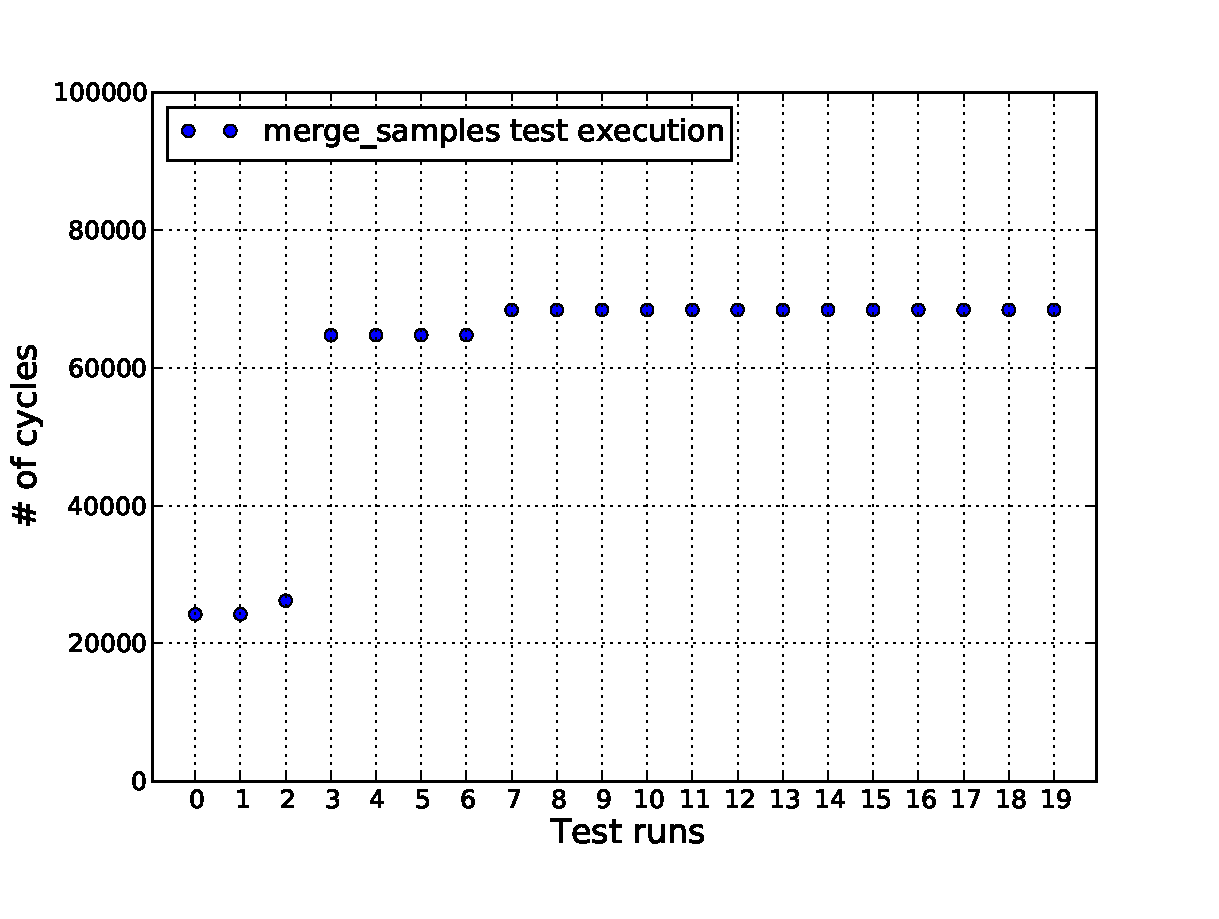
\includegraphics[width=4in]{q3_2_merge_samples}
  \caption
  {Measurements for \texttt{merge\_samples()}}
	\label{fig:mergeSamples}
\end{figure}

\end{itemize}

\subsection{Listings}
\subsubsection{ait\_merge\_samples.ais}
\lstset{ %
  language=python,                 	   % the language of the code
  backgroundcolor=\color{white},   % choose the background color; you must add \usepackage{color} or \usepackage{xcolor}
  basicstyle=\footnotesize\ttfamily,        % the size of the fonts that are used for the code
  breakatwhitespace=false,         % sets if automatic breaks should only happen at whitespace
  breaklines=true,                 % sets automatic line breaking
  captionpos=b,                    % sets the caption-position to bottom
  commentstyle=\color{mygray},    % comment style
  deletekeywords={...,in},            % if you want to delete keywords from the given language
  escapeinside={\%*}{*)},          % if you want to add LaTeX within your code
  extendedchars=true,              % lets you use non-ASCII characters; for 8-bits encodings only, does not work with UTF-8
  %frame=single,                    % adds a frame around the code
  keepspaces=true,                 % keeps spaces in text, useful for keeping indentation of code (possibly needs columns=flexible)
  keywordstyle=\bfseries\color{blue},       % keyword style
  morekeywords={*,...,instruction,loop, entered, with, max, flow, label},            % if you want to add more keywords to the set
  numbers=left,                    % where to put the line-numbers; possible values are (none, left, right)
  numbersep=5pt,                   % how far the line-numbers are from the code
  numberstyle=\tiny\color{mygray}, % the style that is used for the line-numbers
  rulecolor=\color{black},         % if not set, the frame-color may be changed on line-breaks within not-black text (e.g. comments (green here))
  showspaces=false,                % show spaces everywhere adding particular underscores; it overrides 'showstringspaces'
  showstringspaces=false,          % underline spaces within strings only
  showtabs=false,                  % show tabs within strings adding particular underscores
  stepnumber=1,                    % the step between two line-numbers. If it's 1, each line will be numbered
  stringstyle=\color{mymauve},     % string literal style
  tabsize=2,                       % sets default tabsize to 2 spaces
  %extendedchars=true,
  %aboveskip={1.5\baselineskip},
  %columns=fixed, upquote=true,
  %title=\lstname                   % show the filename of files included with \lstinputlisting; also try caption instead of title
}


\lstinputlisting{src/aiTmergeSamples.ais}

\subsubsection{task.c:merge\_samples()}
\lstset{ %
  language=C,                 	   % the language of the code
  backgroundcolor=\color{white},   % choose the background color; you must add \usepackage{color} or \usepackage{xcolor}
  basicstyle=\footnotesize\ttfamily,        % the size of the fonts that are used for the code
  breakatwhitespace=false,         % sets if automatic breaks should only happen at whitespace
  breaklines=true,                 % sets automatic line breaking
  captionpos=b,                    % sets the caption-position to bottom
  commentstyle=\color{mygreen},    % comment style
  deletekeywords={...},            % if you want to delete keywords from the given language
  escapeinside={\%*}{*)},          % if you want to add LaTeX within your code
  extendedchars=true,              % lets you use non-ASCII characters; for 8-bits encodings only, does not work with UTF-8
  %frame=single,                    % adds a frame around the code
  keepspaces=true,                 % keeps spaces in text, useful for keeping indentation of code (possibly needs columns=flexible)
  keywordstyle=\bfseries\color{blue},       % keyword style
  morekeywords={*,...},            % if you want to add more keywords to the set
  numbers=left,                    % where to put the line-numbers; possible values are (none, left, right)
  numbersep=5pt,                   % how far the line-numbers are from the code
  numberstyle=\tiny\color{mygray}, % the style that is used for the line-numbers
  rulecolor=\color{black},         % if not set, the frame-color may be changed on line-breaks within not-black text (e.g. comments (green here))
  showspaces=false,                % show spaces everywhere adding particular underscores; it overrides 'showstringspaces'
  showstringspaces=false,          % underline spaces within strings only
  showtabs=false,                  % show tabs within strings adding particular underscores
  stepnumber=1,                    % the step between two line-numbers. If it's 1, each line will be numbered
  stringstyle=\color{mymauve},     % string literal style
  tabsize=2,                       % sets default tabsize to 2 spaces
  %extendedchars=true,
  %aboveskip={1.5\baselineskip},
  %columns=fixed, upquote=true,
  %title=\lstname                   % show the filename of files included with \lstinputlisting; also try caption instead of title
}


\lstinputlisting{src/mergeSamples.c}

%------------------------------------------------------------------
\newpage
\section{Problem 4}

\subsection{Problem Statement}
\label{problem:4}

Next, analyze the \texttt{fft()} function called in \texttt{task.c}. Try to
find loop bounds for the Fast Fourier Transform implementation
(\texttt{fixedpoint.c:fp\_radix2fft\_withscaling()}) first, and add a flow
constraint relating the execution frequency of the inner loop's body with
the function's execution frequency.

\begin{itemize}

\item[Q1:]
  Describe and justify the flow facts found for
  \texttt{fp\_radix2fft\_withscaling}, and \texttt{fft}.

\item[Q2:]
  What is the maximum execution time observed for this function? What
  is the analyzed WCET?

\item[Q3:]
  For the FFT implementation \texttt{fp\_radix2fft\_withscaling}, is it safe to
  use the loop iteration counts observed during a test run? Justify your
  answer.

\item[Hint:]
  For measurements, you might want to rely on or start with the test
  implementation \texttt{main.c:test\_fft()}

\end{itemize}


\subsection{Solution}
\begin{itemize}
\item[A1:] 

Function \texttt{fp\_radix2fft\_withscaling} represents a classical implementation of Fast Fourier Transform algorithm.
This algorithm can be implemented in hardware.
This claim can be easily checked by inspecting the code.
A feature of these kind of algorithms is that the function code can be fully unfolded in a plain linear program, i.e. control flow does not depend on the input data.
We treat function arguments \texttt{n} and \texttt{t} as parameters of the algorithm.
In our problem they are constant: $n=64$, $t=\log_2 n = 6$.

For every loop in \texttt{fp\_radix2fft\_withscaling} it is true that the loop variable does not change inside the loop body.
The outer loop executes exactly $t=6$ times.
The two inner loops execute at most $2^5=32$ times each during a single iteration of the outer loop.
Moreover, the bounds of the two inner loops are set exclusively in the outer loop and in the way that there is a strict relation between them.
Indeed, if the current iteration of the outer loop is $q$, then the number of iterations of the inner loops are exactly $2^{t-q}=2^{6-q}$ and $2^{q-1}$.
The number of the most inner loop body executions is exactly $2^{6-q}\cdot2^{q-1}=2^5$ in the current iteration of the outer loop.
In total, the most inner loop body is executed exactly $t\cdot2^{t-1}=6\cdot2^5=192$ times.
The middle loop (the inner loop with the loop variable \texttt{k}) body execution count depends on the value of \texttt{r} which is constant during each outer loop iteration, but decreases after each outer loop iteration.
In total, the middle loop body is executed exactly $\sum_{q=1}^t 2^{t-q} = 2^t -1 = 2^6-1 = 63$ times.

Function \texttt{fp\_radix2fft\_withscaling} performs two calls of the function \texttt{bitreverse} before entering the loops.
However, \texttt{bitreverse} has the same properties as \texttt{fp\_radix2fft\_withscaling} itself: the control flow does not depend on the data, the loops can be fully unfolded and the function can be implemented in hardware.
We treat a constant array, passed to the function, as a parameter, but not an input, since it is always the same for all function calls with the sane value of \texttt{n}.
In fact, \texttt{bitreverse} represents constant permutation or fixed routing in hardware.
Clearly, the loop is always executed $n=64$ times, but the body of the \texttt{if} operator is expected to be executed significantly smaller number of times.
Although, it is difficult to compute this number analytically, the function will always follow the same control flow.
With a single run of the function we found that the body of the \texttt{if} operator is executed 28 times.

%TODO
\fbox{TODO: Describe \texttt{fft}}

\item[A2:] 
  Since \texttt{test\_fft()} provides only one execution of
  \texttt{fft} we modified  \texttt{merge\_samples()} to
  perform more elaborate testing. We invoke \texttt{fft} 20 times
  with different \texttt{input\_buffer}.
  The measurements for \texttt{fp\_radix2fft\_withscaling} and \texttt{fft} are
  shown in the Figure~\ref{fig:fft_radix}.
  
  WCET analysis with \texttt{a3patmos} gives the following results:

  $$\text{WCET}_{\text{fp\_radix2fft\_withscaling}} = 3\enskip 496\enskip 504$$
  $$\text{WCET}_{\text{fft}} = 4\enskip 919\enskip 107$$

\begin{figure}%[hb!]
\centering
  \begin{minipage}{0.8\textwidth}
	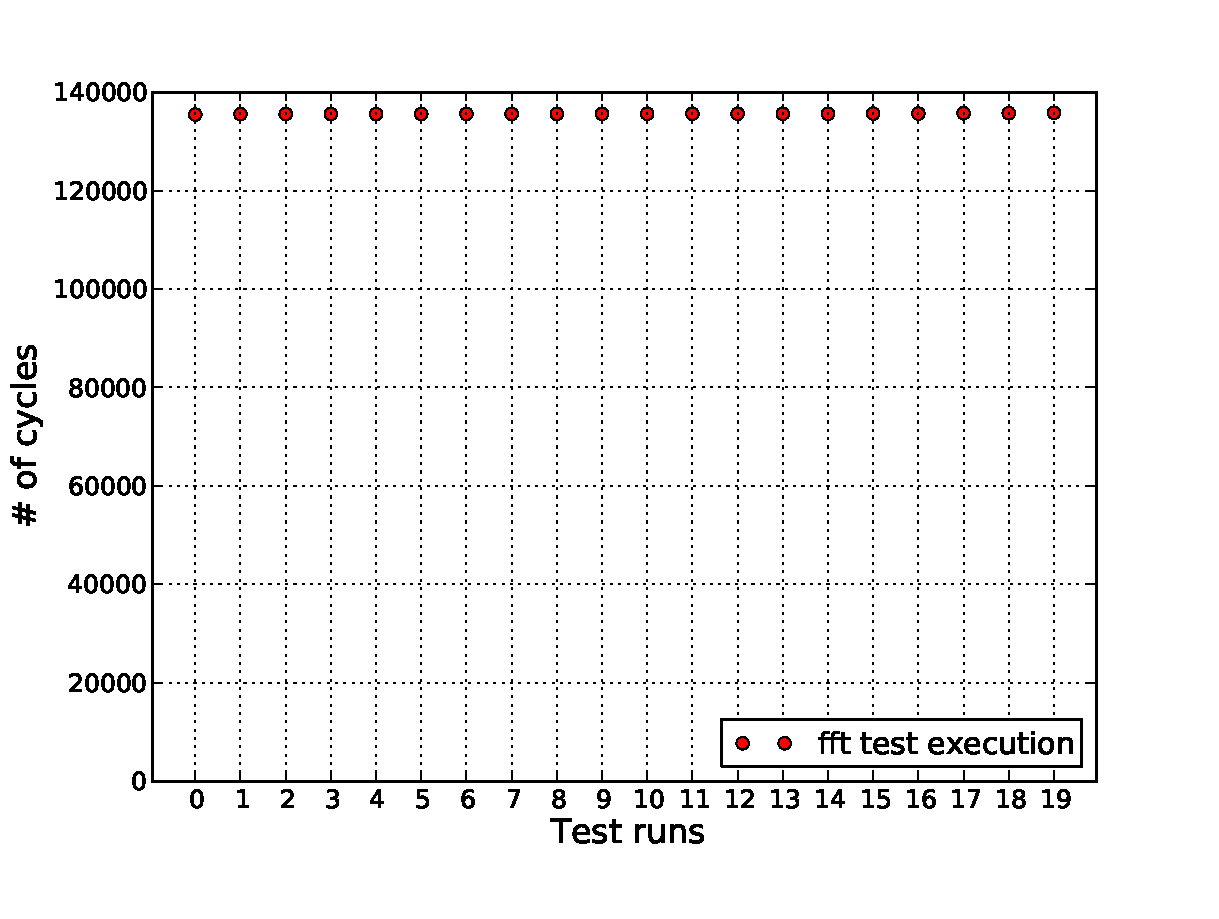
\includegraphics[width=4in]{fft_test}
  \end{minipage}
  \begin{minipage}{0.8\textwidth}
	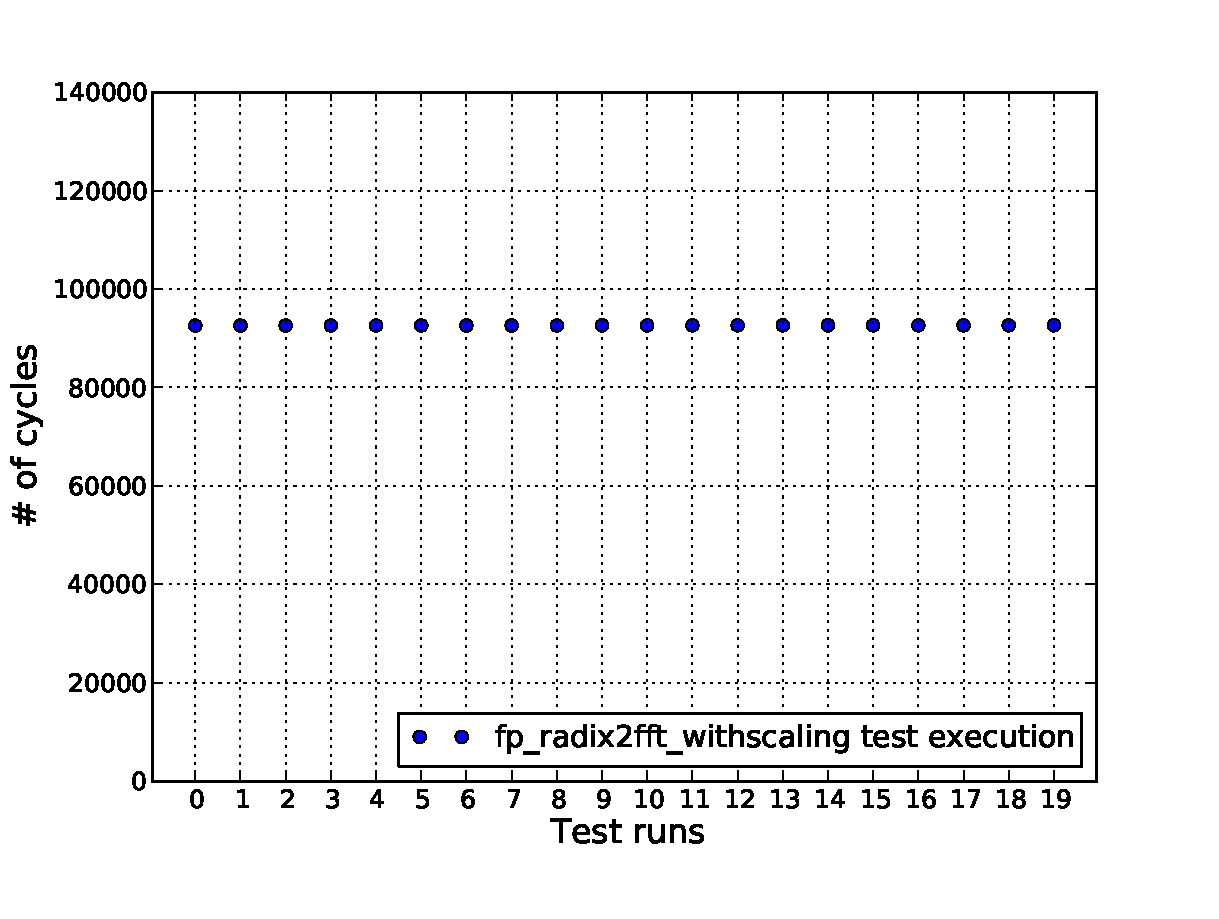
\includegraphics[width=4in]{radix2fft}
  \end{minipage}
\caption{Measurements of execution time}
\label{fig:fft_radix}
\end{figure}


\item[A3:]
It is absolutely safe to use for analysis the loop iteration counts observed during a test run of \texttt{fp\_radix2fft\_withscaling}.
The reason is given in the section A1 above.

\end{itemize}

\subsection{Listings}

\subsubsection{ait\_fft.ais}
\lstset{ %
  language=python,                 	   % the language of the code
  backgroundcolor=\color{white},   % choose the background color; you must add \usepackage{color} or \usepackage{xcolor}
  basicstyle=\footnotesize\ttfamily,        % the size of the fonts that are used for the code
  breakatwhitespace=false,         % sets if automatic breaks should only happen at whitespace
  breaklines=true,                 % sets automatic line breaking
  captionpos=b,                    % sets the caption-position to bottom
  commentstyle=\color{mygray},    % comment style
  deletekeywords={...,in},            % if you want to delete keywords from the given language
  escapeinside={\%*}{*)},          % if you want to add LaTeX within your code
  extendedchars=true,              % lets you use non-ASCII characters; for 8-bits encodings only, does not work with UTF-8
  %frame=single,                    % adds a frame around the code
  keepspaces=true,                 % keeps spaces in text, useful for keeping indentation of code (possibly needs columns=flexible)
  keywordstyle=\bfseries\color{blue},       % keyword style
  morekeywords={*,...,instruction,loop, entered, with, max, flow, label},            % if you want to add more keywords to the set
  numbers=left,                    % where to put the line-numbers; possible values are (none, left, right)
  numbersep=5pt,                   % how far the line-numbers are from the code
  numberstyle=\tiny\color{mygray}, % the style that is used for the line-numbers
  rulecolor=\color{black},         % if not set, the frame-color may be changed on line-breaks within not-black text (e.g. comments (green here))
  showspaces=false,                % show spaces everywhere adding particular underscores; it overrides 'showstringspaces'
  showstringspaces=false,          % underline spaces within strings only
  showtabs=false,                  % show tabs within strings adding particular underscores
  stepnumber=1,                    % the step between two line-numbers. If it's 1, each line will be numbered
  stringstyle=\color{mymauve},     % string literal style
  tabsize=2,                       % sets default tabsize to 2 spaces
  %extendedchars=true,
  %aboveskip={1.5\baselineskip},
  %columns=fixed, upquote=true,
  %title=\lstname                   % show the filename of files included with \lstinputlisting; also try caption instead of title
}


\lstinputlisting{src/aiTfft.ais}

\subsubsection{fft}
\lstset{ %
  language=C,                 	   % the language of the code
  backgroundcolor=\color{white},   % choose the background color; you must add \usepackage{color} or \usepackage{xcolor}
  basicstyle=\footnotesize\ttfamily,        % the size of the fonts that are used for the code
  breakatwhitespace=false,         % sets if automatic breaks should only happen at whitespace
  breaklines=true,                 % sets automatic line breaking
  captionpos=b,                    % sets the caption-position to bottom
  commentstyle=\color{mygreen},    % comment style
  deletekeywords={...},            % if you want to delete keywords from the given language
  escapeinside={\%*}{*)},          % if you want to add LaTeX within your code
  extendedchars=true,              % lets you use non-ASCII characters; for 8-bits encodings only, does not work with UTF-8
  %frame=single,                    % adds a frame around the code
  keepspaces=true,                 % keeps spaces in text, useful for keeping indentation of code (possibly needs columns=flexible)
  keywordstyle=\bfseries\color{blue},       % keyword style
  morekeywords={*,...},            % if you want to add more keywords to the set
  numbers=left,                    % where to put the line-numbers; possible values are (none, left, right)
  numbersep=5pt,                   % how far the line-numbers are from the code
  numberstyle=\tiny\color{mygray}, % the style that is used for the line-numbers
  rulecolor=\color{black},         % if not set, the frame-color may be changed on line-breaks within not-black text (e.g. comments (green here))
  showspaces=false,                % show spaces everywhere adding particular underscores; it overrides 'showstringspaces'
  showstringspaces=false,          % underline spaces within strings only
  showtabs=false,                  % show tabs within strings adding particular underscores
  stepnumber=1,                    % the step between two line-numbers. If it's 1, each line will be numbered
  stringstyle=\color{mymauve},     % string literal style
  tabsize=2,                       % sets default tabsize to 2 spaces
  %extendedchars=true,
  %aboveskip={1.5\baselineskip},
  %columns=fixed, upquote=true,
  %title=\lstname                   % show the filename of files included with \lstinputlisting; also try caption instead of title
}


\lstinputlisting{src/fft.c}

\subsubsection{fp\_radix2fft\_withscaling}
\lstset{ %
  language=C,                 	   % the language of the code
  backgroundcolor=\color{white},   % choose the background color; you must add \usepackage{color} or \usepackage{xcolor}
  basicstyle=\footnotesize\ttfamily,        % the size of the fonts that are used for the code
  breakatwhitespace=false,         % sets if automatic breaks should only happen at whitespace
  breaklines=true,                 % sets automatic line breaking
  captionpos=b,                    % sets the caption-position to bottom
  commentstyle=\color{mygreen},    % comment style
  deletekeywords={...},            % if you want to delete keywords from the given language
  escapeinside={\%*}{*)},          % if you want to add LaTeX within your code
  extendedchars=true,              % lets you use non-ASCII characters; for 8-bits encodings only, does not work with UTF-8
  %frame=single,                    % adds a frame around the code
  keepspaces=true,                 % keeps spaces in text, useful for keeping indentation of code (possibly needs columns=flexible)
  keywordstyle=\bfseries\color{blue},       % keyword style
  morekeywords={*,...},            % if you want to add more keywords to the set
  numbers=left,                    % where to put the line-numbers; possible values are (none, left, right)
  numbersep=5pt,                   % how far the line-numbers are from the code
  numberstyle=\tiny\color{mygray}, % the style that is used for the line-numbers
  rulecolor=\color{black},         % if not set, the frame-color may be changed on line-breaks within not-black text (e.g. comments (green here))
  showspaces=false,                % show spaces everywhere adding particular underscores; it overrides 'showstringspaces'
  showstringspaces=false,          % underline spaces within strings only
  showtabs=false,                  % show tabs within strings adding particular underscores
  stepnumber=1,                    % the step between two line-numbers. If it's 1, each line will be numbered
  stringstyle=\color{mymauve},     % string literal style
  tabsize=2,                       % sets default tabsize to 2 spaces
  %extendedchars=true,
  %aboveskip={1.5\baselineskip},
  %columns=fixed, upquote=true,
  %title=\lstname                   % show the filename of files included with \lstinputlisting; also try caption instead of title
}


\lstinputlisting{src/fpRadix2fftWithscaling.c}

\subsubsection{bitreverse}
\lstset{ %
  language=C,                 	   % the language of the code
  backgroundcolor=\color{white},   % choose the background color; you must add \usepackage{color} or \usepackage{xcolor}
  basicstyle=\footnotesize\ttfamily,        % the size of the fonts that are used for the code
  breakatwhitespace=false,         % sets if automatic breaks should only happen at whitespace
  breaklines=true,                 % sets automatic line breaking
  captionpos=b,                    % sets the caption-position to bottom
  commentstyle=\color{mygreen},    % comment style
  deletekeywords={...},            % if you want to delete keywords from the given language
  escapeinside={\%*}{*)},          % if you want to add LaTeX within your code
  extendedchars=true,              % lets you use non-ASCII characters; for 8-bits encodings only, does not work with UTF-8
  %frame=single,                    % adds a frame around the code
  keepspaces=true,                 % keeps spaces in text, useful for keeping indentation of code (possibly needs columns=flexible)
  keywordstyle=\bfseries\color{blue},       % keyword style
  morekeywords={*,...},            % if you want to add more keywords to the set
  numbers=left,                    % where to put the line-numbers; possible values are (none, left, right)
  numbersep=5pt,                   % how far the line-numbers are from the code
  numberstyle=\tiny\color{mygray}, % the style that is used for the line-numbers
  rulecolor=\color{black},         % if not set, the frame-color may be changed on line-breaks within not-black text (e.g. comments (green here))
  showspaces=false,                % show spaces everywhere adding particular underscores; it overrides 'showstringspaces'
  showstringspaces=false,          % underline spaces within strings only
  showtabs=false,                  % show tabs within strings adding particular underscores
  stepnumber=1,                    % the step between two line-numbers. If it's 1, each line will be numbered
  stringstyle=\color{mymauve},     % string literal style
  tabsize=2,                       % sets default tabsize to 2 spaces
  %extendedchars=true,
  %aboveskip={1.5\baselineskip},
  %columns=fixed, upquote=true,
  %title=\lstname                   % show the filename of files included with \lstinputlisting; also try caption instead of title
}


\lstinputlisting{src/bitreverse.c}


%------------------------------------------------------------------
\newpage
\section{Problem 5}

\subsection{Problem Statement}
\label{problem:5}
The final goal is to analyze the WCET of \texttt{task.c:task()}.

\begin{itemize}

\item[Q1:]
  First, calculate the WCET of \texttt{check\_sin} and \texttt{check\_square}.
  Then, try to give a rough estimate on the WCET by combining the WCET's of
  \texttt{merge\_samples}, \texttt{fft}, \texttt{check\_sin} and
  \texttt{check\_square}. Clearly state how you combined the WCETs, and compare
  the resulting value with the maximum observed execution time of these
  functions, combined in the same way.

\item[Q2:]
  Add a flow fact for the indirect call in \texttt{task}, calculate the WCET of
  \texttt{task}, and compare it to the maximum execution time observed.

\end{itemize}


\subsection{Solution}
% TODO

\subsection{Listings}
% TODO

%------------------------------------------------------------------
\newpage
\section{Reflections}

%\subsection{Problem Statement}
\label{problem:6}

Answer the following questions:

\begin{itemize}

\item[Q1:]
  How much time did you spend writing annotations and analyzing the code?
  Was it less or more than you expected?

\item[Q2:]
  What problems did you encounter during this assignment?

\item[Q3:]
  As you learned, sometimes it is necessary to annotate the assembly code.
  Why? What problems can you see because of this?

\end{itemize}


\subsection{Answers}
\begin{itemize}

\item[A1:]
  We have spent quite some time doing the lab, and (at least for me)
  it was more than expected. Writing annotations will not take much
  time for a person familiar with the framework and the work flow, but
  in order to understand how all the 

\item[A2:]
TODO

\item[A3:]
TODO

\end{itemize}


\end{document}

